\documentclass[sigplan,screen,review,anonymous]{acmart}

\settopmatter{printfolios=false}
\renewcommand{\shortauthors}{Anonymous Author(s)}
\citestyle{acmnumeric}

\usepackage{graphicx}
\usepackage{xcolor}
\usepackage{xspace}
\usepackage{hyperref}
\usepackage{booktabs}
\usepackage{array}
\usepackage{tikz}
\usepackage{pgfplots}
\usepackage{placeins}
\usepackage{stfloats}
\usetikzlibrary{patterns,plotmarks}
\usepgfplotslibrary{groupplots}
\usepgfplotslibrary{fillbetween}
\pgfplotsset{compat=1.18}

\setlength{\textfloatsep}{8pt plus 2pt minus 2pt}
\setlength{\floatsep}{6pt plus 2pt minus 2pt}
\setlength{\intextsep}{6pt plus 2pt minus 2pt}
\setlength{\dbltextfloatsep}{8pt plus 2pt minus 2pt}
\setlength{\dblfloatsep}{6pt plus 2pt minus 2pt}
\renewcommand{\topfraction}{0.95}
\renewcommand{\dbltopfraction}{0.95}
\renewcommand{\textfraction}{0.05}
\renewcommand{\floatpagefraction}{0.85}
\renewcommand{\dblfloatpagefraction}{0.85}

\graphicspath{{img/}}

\newcommand{\system}{\textsc{VeriEdge}\xspace}
\newcommand{\suppRiskCompositionWidth}{0.9\linewidth}
\newcommand{\suppDeliveryScalingWidth}{1\linewidth}
\newcommand{\suppLiveStoreWidth}{1\linewidth}
\newcommand{\suppProjScalarStabilityWidth}{1\linewidth}
\newcommand{\suppProjScalarBoundaryWidth}{1\linewidth}
\newcommand{\suppStrengthSweepWidth}{1\linewidth}
\newcommand{\suppPayloadLatencyWidth}{1\linewidth}
\newcommand{\suppPolicyCompareWidth}{1\linewidth}

\begin{document}

\title[Supplementary Evaluation Results for VeriEdge]{Supplementary Evaluation Results for%
\texorpdfstring{\\}{ }%
\texorpdfstring{\system}{VeriEdge}: Verifiability-Constrained Placement for Heterogeneous Edge LLM Inference}

\author{Anonymous Author(s)}
\affiliation{
  \institution{Anonymous Institution(s)}
  \country{}
}

\ccsdesc[500]{Computer systems organization~Dependable and fault-tolerant systems}
\ccsdesc[300]{Security and privacy~Distributed systems security}
\keywords{edge AI, decentralized inference, heterogeneous systems, verification, orchestration}

\acmConference[EuroSys '27]{European Conference on Computer Systems}{April 19--23, 2027}{Rabat, Morocco}

\maketitle
\thispagestyle{empty}
\pagestyle{empty}
\raggedbottom

\phantomsection
\label{app:eval-supplement}

This supplement provides evaluation details that support the main paper without
extending its claims. It reports the measured verifier-profile matrix,
placement replay inputs, selective-delivery scaling, sketch robustness checks,
known sketch blind spots, overhead breakdowns, and full policy-composition
views.

\section{Measured Verifier Profiles Used by Placement Replay}
\label{app:profile-matrix}

Table~\ref{tab:app-profile-matrix} reports the verifier-profile matrix used by
the closed-loop placement replay. Each row is a profile key: stack pair, sketch
mode, and checked C1--C3 boundaries. The risk class is the descriptive class
used by the risk-composition plots; task admission still applies the explicit
\(\alpha,\beta,S^{\max},C^{\max}\) feasibility test. Scale TPR is reported as a
diagnostic for the cosine-sketch blind spot, while admission uses held-out
honest FPR and primary material-tamper TPR.


\section{Placement Replay Inputs and Policy Semantics}
\label{app:placement-replay-config}

The replay is a controlled decision replay rather than a live marketplace
trace. It fixes three inputs: the verifier-profile matrix in
Table~\ref{tab:app-profile-matrix}, a candidate-placement table, and a workload
table. The candidate table contains 13 placements: one homogeneous F/F control
and 12 heterogeneous LAN/WAN variants over A/B, A/B-RTXint8, A/C, A/D, B/D,
and E/F. Each candidate records a provider group, a C1--C3 shard map, a
stack-pair label, network and execution latency estimates, availability cost,
reputation, capacity feasibility, and backend-mix class. The workload table
contains 400 records: 200 evaluation prompts replayed as a low-pressure
single-arrival workload and the same 200 prompts replayed as a queued-8 burst
workload. Table~\ref{tab:app-placement-replay-config} summarizes these fixed
replay inputs.


Table~\ref{tab:app-placement-policy-exact} reports the queued-8 replay numbers
summarized in the main paper. The main text uses the figure and key deltas for
the placement narrative; this table preserves exact policy metrics for
comparison.


For each task and policy, the replay first filters candidates by capacity and
group-size bounds. A candidate and sketch choice then looks up its measured
profile row. The selected choice is admissible when
\(\mathrm{FPR}\le\alpha\), primary-material \(\mathrm{TPR}\ge\beta\), trace
bytes are within \(S^{\max}\), and challenge-time verifier latency is within
\(C^{\max}\). If a policy selects a candidate whose profile violates any of
these checks, the admitted task contributes to infeasible usage. False-dispute
risk is computed as \(0.10\times\mathrm{FPR}\) for the selected profile.
Expected challenge cost is computed analogously as \(0.10\) times the measured
honest verifier latency.

The policy families differ in when they use these profiles. Network-aware
baselines first choose the lowest-latency candidate from network and execution
estimates, then attach a fixed sketch. Risk-constrained policies apply the
hard verifiability admission test before ranking. Adaptive-verifier policies
choose the smallest feasible sketch for a selected candidate, or jointly choose
a candidate and sketch under the same feasibility test. Queue-aware policies
add current candidate wait time,
\(\max(0,\mathsf{busyUntil}-\mathsf{arrival})\), to the placement score before
choosing a candidate. Replay latency is modeled service time plus queue wait,
and goodput is the number of admitted tasks divided by final completion time.

\section{Risk Composition Behind Placement Decisions}
\label{app:placement-risk-composition}

Figure~\ref{fig:app-risk-composition} decomposes which verifier-profile risk
classes are actually selected by each placement policy. This view complements
the main paper's placement-frontier plots: latency-oriented network and
queue-aware policies can improve modeled service time or queueing behavior
while still selecting profile keys that violate the task's FPR/TPR target.
Risk-constrained and adaptive-verifier policies remove those choices before
task disclosure, either by filtering the placement or by upgrading the sketch
mode. The same pattern appears in both arrival regimes. At
\(\alpha=0.10\), network-aware projcos4 has infeasible usage \(1.000\) in
both the single and queued-8 replay, while risk-constrained and adaptive
variants keep infeasible usage at \(0.000\). In the queue-aware replay,
queue-aware network placement reaches the highest goodput, but still uses
infeasible profile keys for \(93.5\%\) of admitted tasks; queue-aware adaptive
placement keeps infeasible usage at zero while preserving nearly the same
goodput.


\section{Selective Delivery and Placement-Defined Disclosure}
\label{app:delivery-scaling}

The main paper reports the central 100MB selective-delivery readout. Here we
include the exact modeled LAN/WAN medians in
Table~\ref{tab:app-delivery-sweep-exact} and corresponding curves in
Figure~\ref{fig:app-delivery-scaling}. The experiment compares replicated
payload delivery (RPD), which sends one full encrypted payload per selected
provider, against privacy-preserving delivery (PPD), which publishes one
encrypted object and releases small locator-and-key packages after the
placement commitment. Both modes encrypt the payload; the difference is
whether requester-side payload transfer scales with selected group size.



\paragraph{Live local-store validation.}
The LAN/WAN sweep is a calibrated delivery-path model, so we also ran a local
store supplement to validate the disclosure-path assumptions. Each of the 240
local-store runs created a fresh ciphertext, derived the object key from the
actual SHA-256 content hash, had providers fetch the object, and hash-checked
the fetched ciphertext. This supplement is not used as the LAN/WAN latency
source; it rules out cache reuse and confirms that the measured PPD path uses
fresh stored objects and targeted access material. Table~\ref{tab:app-live-store}
reports the exact local-store medians.



\section{Projected-Scalar Bridge Stability}
\label{app:projscalar-stability}

Figure~\ref{fig:app-projscalar-stability} checks whether the
projscalar1\_abs bridge in the main evaluation is an artifact of one random
seed. Across A/B, A/B-RTXint8, A/C, A/D, B/D, and E/F with five seeds, every
selected operating point remains admissible under the
\(\alpha=0.10,\beta=0.90\) profile, with mean held-out FPR \(0.0073\), max FPR
\(0.025\), and minimum primary-material TPR \(1.000\). This supports using the
sketch as a norm-sensitive companion to projected-token cosine TSTC. It is a
diagnostic and hybrid-verifier component rather than a replacement for
projected-token TSTC.


\section{Norm-Sensitive Bridge Boundary}
\label{app:projscalar-boundary}

Figure~\ref{fig:app-projscalar-boundary} expands the projected-scalar bridge.
The bridge detects scale perturbations that cosine-only projected-token
sketches miss because it keeps norm information. However, a projection-aware
null-space attack can avoid the one-dimensional projection. This is the
boundary used in the main paper: norm-sensitive projections are useful hybrid
components, not adaptive cryptographic guarantees.


\section{Material-Tamper Coverage and Cosine Blind Spot}
\label{app:strength-sweep}

Figure~\ref{fig:app-strength-sweep} varies perturbation strength for the
material-tamper study. Projcos4 detects Gaussian perturbations across the
tested strengths, while scale-only perturbations remain undetected. This
matches the TSTC mechanism: projected-token cosine sketches retain directional
geometry but deliberately discard most norm information.

Table~\ref{tab:app-material-tamper-exact} gives the exact A/B and B/D
attack-family TPRs summarized by the main paper's material-tamper figure.


Table~\ref{tab:app-output-affecting} summarizes the output-affecting subset
across six stack pairs. It separates attacks that merely perturb checkpoint
statistics from attacks that change the next-token neighborhood. Directional
attacks remain detected by projcos4 on the output-affecting subset, while
scale perturbations remain the cosine-only blind spot even when they affect
the output neighborhood.



\section{Checkpoint-Sketch Payload and Challenge-Time Runtime}
\label{app:payload-latency}

Figure~\ref{fig:app-payload-latency} visualizes the payload and latency
numbers summarized in the main paper's verifier-overhead table. Stronger
checkpoint sketches increase reveal payload, but challenge-time verifier
latency remains in the few-millisecond range for the measured implementation.


\section{Full Queued-Workload Policy Metrics}
\label{app:placement-composition}

Figure~\ref{fig:app-placement-policy-compare} returns to the queued-workload
placement replay with the full metric set. Network-aware placement keeps
scalar16 on heterogeneous paths, while risk-constrained and adaptive-verifier
placement upgrade risky profile keys and remove infeasible usage without
changing measured goodput.



\begin{table*}[b]
\centering
\scriptsize
\setlength{\tabcolsep}{4.2pt}
\renewcommand{\arraystretch}{0.94}
\caption{Measured verifier profiles consumed by the closed-loop placement
replay. Each row is a stack-pair/sketch profile key over the three checked
C1--C3 boundaries. B/tr. is the sketch payload per three-checkpoint challenge
trace; TPR\(_p\) is primary material-tamper detection; TPR\(_s\) is
scale-perturbation detection; and ms is honest challenge-time verifier latency
per trace. ``inadjud.'' denotes an inadjudicable profile class; task feasibility
is determined by the explicit admission test.}
\label{tab:app-profile-matrix}
\begin{tabular}{llrrrrrrl}
\toprule
Pair & Sketch & B/tr. & FPR & TPR\(_p\) & TPR\(_s\) & LocAcc & ms & Risk \\
\midrule
A/B & projcos16 & 3072 & 0.120 & 1.000 & 0.000 & 1.000 & 4.04 & medium \\
A/B & projcos4 & 768 & 0.020 & 1.000 & 0.000 & 1.000 & 3.80 & low \\
A/B & projcos8 & 1536 & 0.080 & 1.000 & 0.000 & 1.000 & 3.92 & low \\
A/B & scalar16 & 192 & 0.150 & 0.760 & 0.520 & 0.760 & 3.60 & high \\
A/B & scalar64 & 768 & 0.415 & 0.855 & 0.880 & 0.855 & 3.47 & inadjud. \\
\addlinespace[0.25em]
A/B-RTXint8 & projcos16 & 3072 & 0.080 & 1.000 & 0.000 & 1.000 & 4.04 & low \\
A/B-RTXint8 & projcos4 & 768 & 0.020 & 1.000 & 0.000 & 1.000 & 3.80 & low \\
A/B-RTXint8 & projcos8 & 1536 & 0.035 & 1.000 & 0.000 & 1.000 & 3.92 & low \\
A/B-RTXint8 & scalar16 & 192 & 0.155 & 0.600 & 0.370 & 0.600 & 3.60 & high \\
A/B-RTXint8 & scalar64 & 768 & 0.520 & 0.855 & 0.880 & 0.855 & 3.47 & inadjud. \\
\addlinespace[0.25em]
A/C & projcos16 & 3072 & 0.135 & 1.000 & 0.000 & 1.000 & 4.04 & medium \\
A/C & projcos4 & 768 & 0.045 & 1.000 & 0.000 & 1.000 & 3.80 & low \\
A/C & projcos8 & 1536 & 0.075 & 1.000 & 0.000 & 1.000 & 3.92 & low \\
A/C & scalar16 & 192 & 0.110 & 0.585 & 0.355 & 0.585 & 3.60 & high \\
A/C & scalar64 & 768 & 0.305 & 0.875 & 0.930 & 0.875 & 3.47 & inadjud. \\
\addlinespace[0.25em]
A/D & projcos16 & 3072 & 0.065 & 1.000 & 0.000 & 1.000 & 4.04 & low \\
A/D & projcos4 & 768 & 0.020 & 1.000 & 0.000 & 1.000 & 3.80 & low \\
A/D & projcos8 & 1536 & 0.065 & 1.000 & 0.000 & 1.000 & 3.92 & low \\
A/D & scalar16 & 192 & 0.090 & 0.510 & 0.220 & 0.510 & 3.60 & high \\
A/D & scalar64 & 768 & 0.380 & 0.795 & 0.815 & 0.795 & 3.47 & inadjud. \\
\addlinespace[0.25em]
B/D & projcos16 & 3072 & 0.065 & 1.000 & 0.000 & 1.000 & 4.04 & low \\
B/D & projcos4 & 768 & 0.075 & 1.000 & 0.000 & 1.000 & 3.80 & low \\
B/D & projcos8 & 1536 & 0.075 & 1.000 & 0.000 & 1.000 & 3.92 & low \\
B/D & scalar16 & 192 & 0.245 & 0.950 & 0.720 & 0.950 & 3.60 & high \\
B/D & scalar64 & 768 & 0.590 & 1.000 & 0.995 & 1.000 & 3.47 & inadjud. \\
\addlinespace[0.25em]
E/F & projcos16 & 3072 & 0.030 & 1.000 & 0.005 & 1.000 & 4.04 & low \\
E/F & projcos4 & 768 & 0.105 & 1.000 & 0.060 & 0.985 & 3.80 & medium \\
E/F & projcos8 & 1536 & 0.005 & 1.000 & 0.000 & 1.000 & 3.92 & low \\
E/F & scalar16 & 192 & 0.165 & 1.000 & 1.000 & 1.000 & 3.60 & medium \\
E/F & scalar64 & 768 & 0.615 & 1.000 & 1.000 & 1.000 & 3.47 & inadjud. \\
\addlinespace[0.25em]
F/F & scalar16 & 192 & 0.000 & 1.000 & 1.000 & 1.000 & 3.60 & low \\
F/F & projcos4 & 768 & 0.000 & 1.000 & 1.000 & 1.000 & 3.80 & low \\
F/F & projcos8 & 1536 & 0.000 & 1.000 & 1.000 & 1.000 & 3.92 & low \\
F/F & projcos16 & 3072 & 0.000 & 1.000 & 1.000 & 1.000 & 4.04 & low \\
\bottomrule
\end{tabular}
\end{table*}

\begin{table*}[t]
\centering
\scriptsize
\setlength{\tabcolsep}{4.2pt}
\caption{Fixed inputs for the controlled placement replay used in the main
evaluation.}
\label{tab:app-placement-replay-config}
\begin{tabular}{@{}>{\raggedright\arraybackslash}p{0.28\linewidth}
                >{\raggedright\arraybackslash}p{0.66\linewidth}@{}}
\toprule
Item & Setting \\
\midrule
Candidate placements & 13 total: 1 homogeneous F/F and 12 heterogeneous LAN/WAN variants \\
Stack-pair labels & A/B, A/B-RTXint8, A/C, A/D, B/D, E/F, and F/F control \\
Verifier profiles & 34 measured profile keys, each identified by stack pair and sketch mode over C1--C3 \\
Workload prompts & 200 held-out evaluation prompts \\
Arrival patterns & single: one task every 5.0 s; queued-8: eight tasks every 0.25 s \\
Replay seeds & 5 seeds: 20260513--20260517 \\
Target sweep & \(\alpha\in\{0.05,0.10,0.20\}\), \(\beta=0.90\) \\
Main target & \(\alpha=0.10,\beta=0.90\) \\
Sketch budget & \(S^{\max}=3072\) bytes per three-checkpoint trace \\
Verifier budget & \(C^{\max}=5.0\) ms per challenge \\
Challenge probability & \(0.10\), used for false-risk and challenge-cost expectations \\
Group-size bound & \(1\le |\mathcal{G}|\le 4\); heterogeneous candidates use group size 3 \\
\bottomrule
\end{tabular}
\end{table*}

\begin{table*}[t]
\centering
\scriptsize
\setlength{\tabcolsep}{3.4pt}
\caption{Queued-8 closed-loop placement replay at
\(\alpha=0.10,\beta=0.90\). Risk-constrained hard admission and adaptive
verifier-mode selection remove infeasible profile keys before disclosure;
queue-aware scoring improves modeled latency and goodput, but does not by
itself enforce verifiability. Chal. ms/task is expected challenge-time verifier
cost under challenge probability \(0.10\), and FD risk is expected
false-dispute risk.}
\label{tab:app-placement-policy-exact}
\begin{tabular}{llrrrrrr}
\toprule
Replay & Policy & Med. task s & P95 task s & Goodput & Chal. ms/task & FD risk & Infeas. \\
\midrule
controlled & network-aware, projcos4 & 90.156 & 170.384 & 1.079 & .380 & .0105 & 1.000 \\
controlled & risk-constrained, projcos4 & 91.844 & 173.576 & 1.060 & .380 & .0020 & .000 \\
controlled & network-aware, adaptive & 90.156 & 170.384 & 1.079 & .392 & .0005 & .000 \\
controlled & homogeneous only & 119.301 & 225.498 & .822 & .360 & .0000 & .000 \\
\midrule
queue-aware & network & 5.522 & 9.757 & 12.266 & .360 & .0142 & .935 \\
queue-aware & risk-constrained & 7.004 & 12.714 & 10.392 & .380 & .0033 & .000 \\
queue-aware & adaptive & 5.457 & 9.781 & 12.251 & .380 & .0028 & .000 \\
\bottomrule
\end{tabular}
\end{table*}

\begin{figure*}[t]
\centering
\resizebox{\suppRiskCompositionWidth}{!}{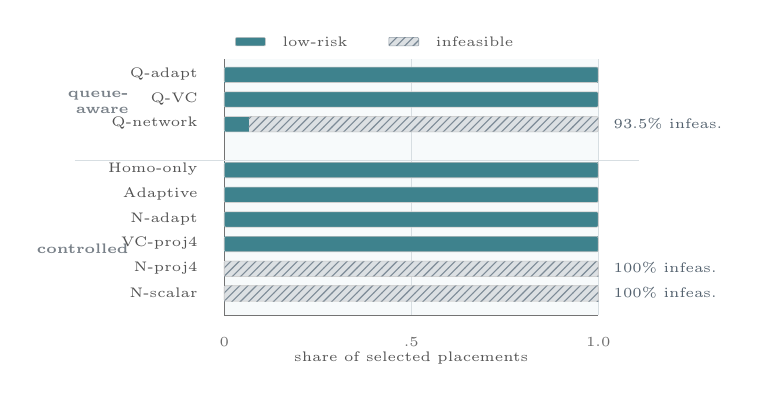
\begin{tikzpicture}[x=4.75cm,y=0.54cm,font=\scriptsize]
\definecolor{veRiskLow}{HTML}{1F6E7A}
\definecolor{veRiskBad}{HTML}{607180}
\definecolor{veRiskGrid}{HTML}{D7DEE2}
\definecolor{veRiskText}{HTML}{525C66}
\definecolor{veRiskPanel}{HTML}{F7FAFB}
\def\barh{0.36}
\def\xleft{-0.40}
\def\xright{1.11}
\def\ytop{7.58}
\def\ybase{1.55}

\path[fill=veRiskPanel,draw=none] (0,\ybase) rectangle (1,\ytop);
\foreach \x/\lab in {0/0,.5/.5,1/1.0} {
	\draw[veRiskGrid,line width=0.22pt] (\x,\ybase) -- (\x,\ytop);
	\node[anchor=north,text=black!58,font=\tiny] at (\x,1.25) {\lab};
}
\draw[black!55,line width=0.33pt] (0,\ybase) -- (1,\ybase);
\draw[black!55,line width=0.33pt] (0,\ybase) -- (0,\ytop);
\node[anchor=north,text=black!68,font=\tiny] at (.5,0.92) {share of selected placements};

\path[fill=veRiskLow!86,draw=black!24,line width=0.2pt,rounded corners=0.35pt]
	(.03,7.88) rectangle (.11,8.08);
\node[anchor=west,text=black!66,font=\tiny] at (.13,7.98) {low-risk};
\path[fill=veRiskBad!22,draw=veRiskBad!70,line width=0.2pt,rounded corners=0.35pt]
	(.44,7.88) rectangle (.52,8.08);
\path[pattern=north east lines,pattern color=veRiskBad!85,draw=none]
	(.44,7.88) rectangle (.52,8.08);
\node[anchor=west,text=black!66,font=\tiny] at (.54,7.98) {infeasible};

\node[anchor=east,text=veRiskText!78,font=\tiny\bfseries,align=right] at (-0.23,6.55) {queue-\\aware};
\node[anchor=east,text=veRiskText!78,font=\tiny\bfseries] at (-0.23,3.10) {controlled};
\draw[veRiskGrid,line width=0.22pt] (\xleft,5.18) -- (\xright,5.18);

\foreach \name/\low/\bad/\yy in {
	Q-adapt/1/0/7.02,
	Q-VC/1/0/6.44,
	Q-network/.065/.935/5.86,
	Homo-only/1/0/4.78,
	Adaptive/1/0/4.20,
	N-adapt/1/0/3.62,
	VC-proj4/1/0/3.04,
	N-proj4/0/1/2.46,
	N-scalar/0/1/1.88
} {
	\node[anchor=east,text=black!68,font=\tiny] at (-0.045,\yy+.20) {\name};
	\path[fill=black!2,draw=black!16,line width=0.18pt,rounded corners=0.45pt]
		(0,\yy) rectangle (1,\yy+\barh);
	\path[fill=veRiskLow!86] (0,\yy) rectangle (\low,\yy+\barh);
	\path[fill=veRiskBad!22] (\low,\yy) rectangle (1,\yy+\barh);
	\path[pattern=north east lines,pattern color=veRiskBad!82] (\low,\yy) rectangle (1,\yy+\barh);
	\draw[draw=black!22,line width=0.2pt,rounded corners=0.45pt]
		(0,\yy) rectangle (1,\yy+\barh);
}

\node[anchor=west,text=veRiskBad!85!black,font=\tiny] at (1.015,6.06) {93.5\% infeas.};
\node[anchor=west,text=veRiskBad!85!black,font=\tiny] at (1.015,2.66) {100\% infeas.};
\node[anchor=west,text=veRiskBad!85!black,font=\tiny] at (1.015,2.08) {100\% infeas.};
\end{tikzpicture}
}
\caption{Selected verifier-profile risk composition in the placement replay.
Network and queue-aware policies can select infeasible profile keys; the
risk-constrained and adaptive policies filter or upgrade those choices before
task disclosure.}
\Description{A TikZ plot showing the selected low-risk, medium-risk,
high-risk, and infeasible verifier-profile composition for controlled and
queue-aware placement policies.}
\label{fig:app-risk-composition}
\end{figure*}

\begin{table*}[t]
\centering
\scriptsize
\setlength{\tabcolsep}{4.2pt}
\caption{Selective-delivery group-size sweep for a 100MB encrypted payload.
Latency is all-providers-ready time under the calibrated LAN/WAN transfer
model; requester egress counts payload-sized transfers sent by the requester.}
\label{tab:app-delivery-sweep-exact}
\begin{tabular}{llrrrrr}
\toprule
Network & \(k\) & RPD med. s & PPD med. s & Med. red. & RPD req. MB & PPD req. MB \\
\midrule
LAN & 1 & 0.864 & 1.719 & \(-99.1\%\) & 100.0 & 100.001 \\
LAN & 2 & 1.715 & 1.720 & \(-0.3\%\) & 200.0 & 100.001 \\
LAN & 4 & 3.417 & 1.719 & \(49.7\%\) & 400.0 & 100.002 \\
LAN & 8 & 6.820 & 1.719 & \(74.8\%\) & 800.0 & 100.005 \\
\midrule
WAN & 1 & 20.088 & 30.259 & \(-50.6\%\) & 100.0 & 100.001 \\
WAN & 2 & 40.099 & 30.272 & \(24.5\%\) & 200.0 & 100.001 \\
WAN & 4 & 80.088 & 30.267 & \(62.2\%\) & 400.0 & 100.002 \\
WAN & 8 & 160.100 & 30.267 & \(81.1\%\) & 800.0 & 100.005 \\
\bottomrule
\end{tabular}
\end{table*}

\begin{figure*}[t]
\centering
\resizebox{\suppDeliveryScalingWidth}{!}{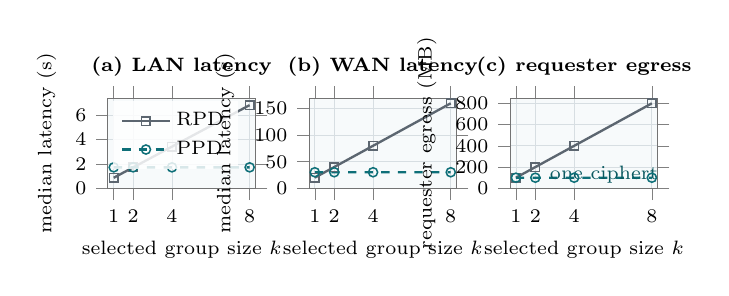
\begin{tikzpicture}
\definecolor{veDeliveryRPD}{HTML}{5C6670}
\definecolor{veDeliveryPPD}{HTML}{0E6F78}
\definecolor{veDeliveryGrid}{HTML}{D7DEE2}
\definecolor{veDeliveryPanel}{HTML}{F7FAFB}
\begin{groupplot}[
	group style={group size=3 by 1,horizontal sep=0.68cm},
	width=0.285\textwidth,
	height=0.225\textwidth,
	xmin=0.7,xmax=8.3,
	xtick={1,2,4,8},
	xlabel={selected group size \(k\)},
	tick label style={font=\scriptsize},
	label style={font=\scriptsize},
	title style={font=\scriptsize\bfseries,yshift=-0.4ex},
	legend style={
		font=\scriptsize,
		draw=none,
		fill=white,
		fill opacity=0.84,
		text opacity=1,
		row sep=0pt,
		cells={anchor=west}
	},
	grid=both,
	major grid style={draw=veDeliveryGrid,line width=0.25pt},
	axis background/.style={fill=veDeliveryPanel},
	axis line style={draw=black!55,line width=0.35pt},
	tick align=outside,
	every axis plot/.append style={line width=0.85pt},
]

\nextgroupplot[
	title={(a) LAN latency},
	ylabel={median latency (s)},
	ymin=0,ymax=7.4,
	ytick={0,2,4,6},
	legend pos=north west,
]
\addplot+[color=veDeliveryRPD,solid,mark=square,mark size=1.55pt,
	mark options={solid,fill=white,draw=veDeliveryRPD,line width=0.55pt}]
	coordinates {(1,0.864) (2,1.715) (4,3.417) (8,6.820)};
\addlegendentry{RPD}
\addplot+[color=veDeliveryPPD,dashed,mark=o,mark size=1.65pt,
	mark options={solid,fill=white,draw=veDeliveryPPD,line width=0.55pt}]
	coordinates {(1,1.719) (2,1.720) (4,1.719) (8,1.719)};
\addlegendentry{PPD}

\nextgroupplot[
	title={(b) WAN latency},
	ylabel={median latency (s)},
	ymin=0,ymax=170,
	ytick={0,50,100,150},
]
\addplot+[color=veDeliveryRPD,solid,mark=square,mark size=1.55pt,
	mark options={solid,fill=white,draw=veDeliveryRPD,line width=0.55pt}]
	coordinates {(1,20.088) (2,40.099) (4,80.088) (8,160.100)};
\addplot+[color=veDeliveryPPD,dashed,mark=o,mark size=1.65pt,
	mark options={solid,fill=white,draw=veDeliveryPPD,line width=0.55pt}]
	coordinates {(1,30.259) (2,30.272) (4,30.267) (8,30.267)};

\nextgroupplot[
	title={(c) requester egress},
	ylabel={requester egress (MB)},
	ymin=0,ymax=850,
	ytick={0,200,400,600,800},
]
\addplot+[color=veDeliveryRPD,solid,mark=square,mark size=1.55pt,
	mark options={solid,fill=white,draw=veDeliveryRPD,line width=0.55pt}]
	coordinates {(1,100.000) (2,200.000) (4,400.000) (8,800.000)};
\addplot+[color=veDeliveryPPD,dashed,mark=o,mark size=1.65pt,
	mark options={solid,fill=white,draw=veDeliveryPPD,line width=0.55pt}]
	coordinates {(1,100.001) (2,100.001) (4,100.002) (8,100.005)};
\node[anchor=west,font=\scriptsize,text=veDeliveryPPD!80!black]
	at (axis cs:2.25,128) {one ciphertext};

\end{groupplot}
\end{tikzpicture}
}
\caption{Placement-defined selective-delivery scaling. RPD becomes dominated
by repeated payload-sized requester transfers as \(k\) grows; PPD keeps
requester egress close to one ciphertext plus small access packages.}
\Description{Three TikZ plots showing LAN latency, WAN latency, and requester
egress for RPD and PPD as selected group size increases.}
\label{fig:app-delivery-scaling}
\end{figure*}

\begin{table*}[t]
\centering
\scriptsize
\setlength{\tabcolsep}{4pt}
\caption{Live local-store validation for a 100MB payload. Latency is
local-store specific; the key result is fresh-object semantics and
requester-egress scaling. PPD store MB is aggregate off-chain-store egress.}
\label{tab:app-live-store}
\begin{tabular}{rrrrrr}
\toprule
\(k\) & RPD med. s & PPD med. s & RPD req. MB & PPD req. MB & PPD store MB \\
\midrule
1 & 0.993 & 1.033 & 100.0 & 100.001 & 100.0 \\
2 & 0.997 & 1.034 & 200.0 & 100.001 & 200.0 \\
4 & 1.048 & 1.046 & 400.0 & 100.003 & 400.0 \\
8 & 1.065 & 1.089 & 800.0 & 100.005 & 800.0 \\
\bottomrule
\end{tabular}
\end{table*}

\begin{figure*}[t]
\centering
\resizebox{\suppLiveStoreWidth}{!}{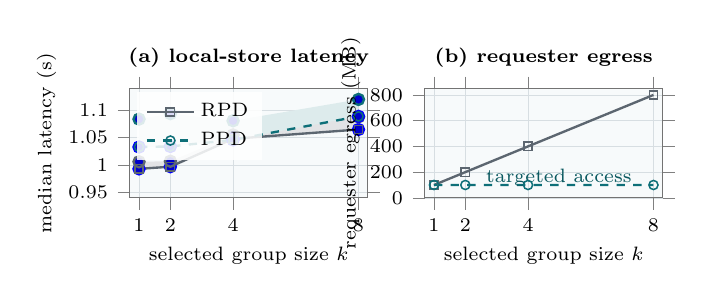
\begin{tikzpicture}
\definecolor{veLiveRPD}{HTML}{5C6670}
\definecolor{veLivePPD}{HTML}{0E6F78}
\definecolor{veLiveGrid}{HTML}{D7DEE2}
\definecolor{veLivePanel}{HTML}{F7FAFB}
\begin{groupplot}[
	group style={group size=2 by 1,horizontal sep=0.72cm},
	width=0.38\textwidth,
	height=0.245\textwidth,
	xmin=0.7,xmax=8.3,
	xtick={1,2,4,8},
	xlabel={selected group size \(k\)},
	xlabel style={yshift=0.15em},
	tick label style={font=\scriptsize},
	label style={font=\scriptsize},
	title style={font=\scriptsize\bfseries,yshift=-0.4ex},
	legend style={
		font=\scriptsize,
		draw=none,
		fill=white,
		fill opacity=0.86,
		text opacity=1,
		row sep=0pt,
		cells={anchor=west}
	},
	grid=both,
	major grid style={draw=veLiveGrid,line width=0.25pt},
	axis background/.style={fill=veLivePanel},
	axis line style={draw=black!55,line width=0.35pt},
	tick align=outside,
	every axis plot/.append style={line width=0.85pt},
]

\nextgroupplot[
	title={(a) local-store latency},
	ylabel={median latency (s)},
	ylabel style={yshift=-0.25em},
	ymin=0.94,ymax=1.14,
	ytick={0.95,1.00,1.05,1.10},
	legend pos=north west,
]
\addplot+[name path=rpdmed,draw=none,forget plot]
	coordinates {(1,0.993) (2,0.997) (4,1.048) (8,1.065)};
\addplot+[name path=rpdp95,color=veLiveRPD,draw=none,forget plot]
	coordinates {(1,1.006) (2,1.007) (4,1.055) (8,1.088)};
\addplot+[veLiveRPD!18,forget plot] fill between[of=rpdmed and rpdp95];
\addplot+[name path=ppdmed,draw=none,forget plot]
	coordinates {(1,1.033) (2,1.034) (4,1.046) (8,1.089)};
\addplot+[name path=ppdp95,color=veLivePPD,draw=none,forget plot]
	coordinates {(1,1.084) (2,1.094) (4,1.081) (8,1.120)};
\addplot+[veLivePPD!14,forget plot] fill between[of=ppdmed and ppdp95];
\addplot+[color=veLiveRPD,solid,mark=square,mark size=1.5pt,
	mark options={solid,fill=white,draw=veLiveRPD,line width=0.55pt}]
	coordinates {(1,0.993) (2,0.997) (4,1.048) (8,1.065)};
\addlegendentry{RPD}
\addplot+[color=veLivePPD,dashed,mark=o,mark size=1.65pt,
	mark options={solid,fill=white,draw=veLivePPD,line width=0.55pt}]
	coordinates {(1,1.033) (2,1.034) (4,1.046) (8,1.089)};
\addlegendentry{PPD}

\nextgroupplot[
	title={(b) requester egress},
	ylabel={requester egress (MB)},
	ylabel style={yshift=-0.35em},
	ymin=0,ymax=850,
	ytick={0,200,400,600,800},
]
\addplot+[color=veLiveRPD,solid,mark=square,mark size=1.5pt,
	mark options={solid,fill=white,draw=veLiveRPD,line width=0.55pt}]
	coordinates {(1,100.000) (2,200.000) (4,400.000) (8,800.000)};
\addplot+[color=veLivePPD,dashed,mark=o,mark size=1.65pt,
	mark options={solid,fill=white,draw=veLivePPD,line width=0.55pt}]
	coordinates {(1,100.001) (2,100.001) (4,100.003) (8,100.005)};
\node[anchor=west,font=\scriptsize,text=veLivePPD!80!black]
	at (axis cs:2.35,155) {targeted access};

\end{groupplot}
\end{tikzpicture}
}
\caption{Live local-store validation of selective delivery. The plot confirms
fresh content-hash object storage and the requester-egress separation between
RPD and PPD; its latency is local-store validation evidence rather than a
WAN/LAN deployment result.}
\Description{A TikZ plot showing live local-store latency and requester egress
for RPD and PPD selective delivery.}
\label{fig:app-live-store}
\end{figure*}

\begin{figure*}[t]
\centering
\resizebox{\suppProjScalarStabilityWidth}{!}{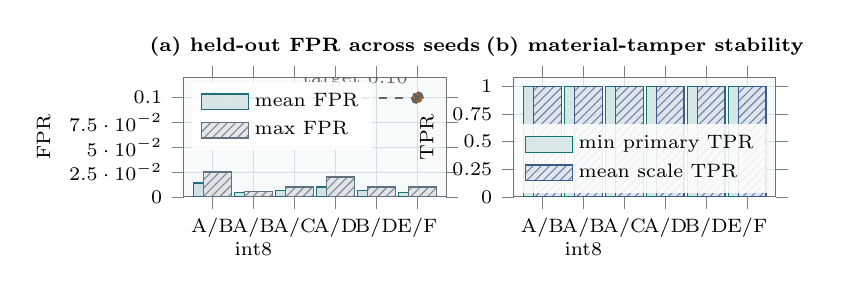
\begin{tikzpicture}
\definecolor{veProjBlue}{HTML}{1F6E7A}
\definecolor{veProjBlueLight}{HTML}{607180}
\definecolor{veProjGreen}{HTML}{0F766E}
\definecolor{veProjAmber}{HTML}{3B5B8A}
\definecolor{veProjGrid}{HTML}{D7DEE2}
\definecolor{veProjPanel}{HTML}{F7FAFB}
\begin{groupplot}[
	group style={group size=2 by 1,horizontal sep=0.86cm},
	width=0.405\textwidth,
	height=0.255\textwidth,
	symbolic x coords={AB,ABint8,AC,AD,BD,EF},
	xtick=data,
	xticklabels={A/B,{A/B\\int8},A/C,A/D,B/D,E/F},
	x tick label style={font=\scriptsize,align=center},
	tick label style={font=\scriptsize},
	label style={font=\scriptsize},
	title style={font=\scriptsize\bfseries,yshift=-0.4ex},
	legend style={
		font=\scriptsize,
		draw=none,
		fill=white,
		fill opacity=0.88,
		text opacity=1,
		row sep=0pt,
		cells={anchor=west}
	},
	enlarge x limits=0.14,
	grid=major,
	major grid style={draw=veProjGrid,line width=0.25pt},
	axis background/.style={fill=veProjPanel},
	axis line style={draw=black!55,line width=0.35pt},
	tick align=outside,
]

\nextgroupplot[
	title={(a) held-out FPR across seeds},
	ylabel={FPR},
	ymin=0,ymax=0.12,
	ytick={0,0.025,0.05,0.075,0.10},
	legend pos=north west,
]
\addplot+[ybar=2.8pt,bar shift=-1.8pt,area legend,mark=none,
	fill=veProjBlue!20,draw=veProjBlue,line width=0.45pt]
	coordinates {
		(AB,0.014) (ABint8,0.004) (AC,0.006)
		(AD,0.010) (BD,0.006) (EF,0.004)
	};
\addlegendentry{mean FPR}
\addplot+[ybar=2.8pt,bar shift=1.8pt,area legend,mark=none,
	fill=veProjBlueLight!18,draw=veProjBlueLight,line width=0.45pt,
	postaction={pattern=north east lines,pattern color=veProjBlueLight!82}]
	coordinates {
		(AB,0.025) (ABint8,0.005) (AC,0.010)
		(AD,0.020) (BD,0.010) (EF,0.010)
	};
\addlegendentry{max FPR}
\addplot+[sharp plot,draw=black!62,dashed,line width=0.75pt,forget plot]
	coordinates {(AB,0.10) (EF,0.10)};
\node[anchor=south east,font=\scriptsize,text=black!62]
	at (axis cs:EF,0.101) {target \(0.10\)};

\nextgroupplot[
	title={(b) material-tamper stability},
	ylabel={TPR},
	ymin=0,ymax=1.08,
	ytick={0,0.25,0.5,0.75,1.0},
	legend pos=south east,
]
\addplot+[ybar=2.8pt,bar shift=-1.8pt,area legend,mark=none,
	fill=veProjGreen!18,draw=veProjGreen,line width=0.45pt]
	coordinates {
		(AB,1.0) (ABint8,1.0) (AC,1.0)
		(AD,1.0) (BD,1.0) (EF,1.0)
	};
\addlegendentry{min primary TPR}
\addplot+[ybar=2.8pt,bar shift=1.8pt,area legend,mark=none,
	fill=veProjAmber!16,draw=veProjAmber,line width=0.45pt,
	postaction={pattern=north east lines,pattern color=veProjAmber!74}]
	coordinates {
		(AB,1.0) (ABint8,1.0) (AC,1.0)
		(AD,1.0) (BD,1.0) (EF,1.0)
	};
\addlegendentry{mean scale TPR}

\end{groupplot}
\end{tikzpicture}
}
\caption{Projected-scalar multiseed stability. The plot summarizes A/B,
A/B-RTXint8, A/C, A/D, B/D, and E/F across five seeds, showing that
projscalar1\_abs remains low-FPR while preserving primary material-tamper
detection.}
\Description{A TikZ plot showing held-out FPR and material-tamper TPR across
five projected-scalar sketch seeds and six stack pairs.}
\label{fig:app-projscalar-stability}
\end{figure*}

\begin{figure*}[t]
\centering
\resizebox{\suppProjScalarBoundaryWidth}{!}{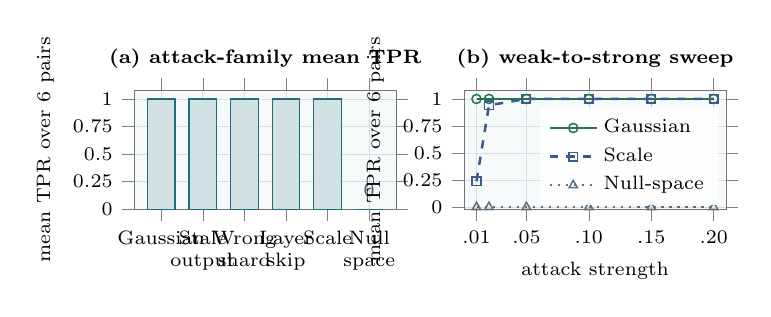
\begin{tikzpicture}
\definecolor{veAttackBlue}{HTML}{1F6E7A}
\definecolor{veAttackGreen}{HTML}{26734D}
\definecolor{veAttackAmber}{HTML}{3B5B8A}
\definecolor{veAttackViolet}{HTML}{607180}
\definecolor{veAttackGrid}{HTML}{D7DEE2}
\definecolor{veAttackPanel}{HTML}{F7FAFB}
\begin{groupplot}[
	group style={group size=2 by 1,horizontal sep=0.86cm},
	width=0.405\textwidth,
	height=0.255\textwidth,
	tick label style={font=\scriptsize},
	label style={font=\scriptsize},
	title style={font=\scriptsize\bfseries,yshift=-0.4ex},
	legend style={
		font=\scriptsize,
		draw=none,
		fill=white,
		fill opacity=0.88,
		text opacity=1,
		row sep=0pt,
		cells={anchor=west}
	},
	grid=major,
	major grid style={draw=veAttackGrid,line width=0.25pt},
	axis background/.style={fill=veAttackPanel},
	axis line style={draw=black!55,line width=0.35pt},
	tick align=outside,
	every axis plot/.append style={line width=0.9pt},
]

\nextgroupplot[
	title={(a) attack-family mean TPR},
	symbolic x coords={Gauss,Stale,Wrong,Skip,Scale,Null},
	xtick=data,
	xticklabels={Gaussian,{Stale\\output},{Wrong\\shard},{Layer\\skip},Scale,{Null\\space}},
	x tick label style={font=\scriptsize,align=center},
	ylabel={mean TPR over 6 pairs},
	ymin=0,ymax=1.08,
	ytick={0,0.25,0.5,0.75,1.0},
	enlarge x limits=0.13,
]
\addplot+[ybar=5.0pt,mark=none,fill=veAttackBlue!20,draw=veAttackBlue,line width=0.45pt]
	coordinates {
		(Gauss,1.0) (Stale,1.0) (Wrong,1.0)
		(Skip,1.0) (Scale,1.0) (Null,0.0)
	};
\node[anchor=south,font=\scriptsize,text=veAttackViolet!80!black]
	at (axis cs:Null,0.03) {0};

\nextgroupplot[
	title={(b) weak-to-strong sweep},
	xlabel={attack strength},
	ylabel={mean TPR over 6 pairs},
	xmin=0.0,xmax=0.21,
	ymin=-0.02,ymax=1.08,
	xtick={0.01,0.05,0.10,0.15,0.20},
	xticklabels={.01,.05,.10,.15,.20},
	ytick={0,0.25,0.5,0.75,1.0},
	legend pos=south east,
]
\addplot+[color=veAttackGreen,solid,mark=o,mark size=1.65pt,
	mark options={solid,fill=white,draw=veAttackGreen,line width=0.55pt}]
	coordinates {
		(0.01,1.0) (0.02,1.0) (0.05,1.0)
		(0.10,1.0) (0.15,1.0) (0.20,1.0)
	};
\addlegendentry{Gaussian}
\addplot+[color=veAttackAmber,dashed,mark=square,mark size=1.55pt,
	mark options={solid,fill=white,draw=veAttackAmber,line width=0.55pt}]
	coordinates {
		(0.01,0.239167) (0.02,0.941667) (0.05,1.0)
		(0.10,1.0) (0.15,1.0) (0.20,1.0)
	};
\addlegendentry{Scale}
\addplot+[color=veAttackViolet,dotted,mark=triangle,mark size=1.75pt,
	mark options={solid,fill=white,draw=veAttackViolet,line width=0.55pt}]
	coordinates {
		(0.01,0.0) (0.02,0.0) (0.05,0.0)
		(0.10,0.0) (0.15,0.0) (0.20,0.0)
	};
\addlegendentry{Null-space}

\end{groupplot}
\end{tikzpicture}
}
\caption{Projected-scalar attack-family and strength-sweep results. The sketch
covers scale perturbations that cosine gaps miss, but exposes the expected
null-space boundary for projection-aware attacks.}
\Description{A TikZ plot showing attack-family TPR and strength-sweep behavior
for the projected-scalar absolute-gap sketch.}
\label{fig:app-projscalar-boundary}
\end{figure*}

\begin{table*}[t]
\centering
\scriptsize
\setlength{\tabcolsep}{2.6pt}
\renewcommand{\arraystretch}{0.92}
\caption{Material-tamper TPR by attack family. Projected-token cosine sketches
detect direction-changing attacks but are weak against direction-preserving
scale perturbations.}
\label{tab:app-material-tamper-exact}
\begin{tabular}{@{}llccccc@{}}
\toprule
Pair & Variant & Gauss. & Cross prompt & Wrong shard & Layer skip & Scale \\
\midrule
A/B & scalar16 & 1.00 & .76 & .76 & .83 & .52 \\
A/B & projcos4 & 1.00 & 1.00 & 1.00 & 1.00 & .00 \\
B/D & scalar16 & 1.00 & .95 & .95 & 1.00 & .72 \\
B/D & projcos4 & 1.00 & 1.00 & 1.00 & 1.00 & .00 \\
\bottomrule
\end{tabular}
\end{table*}

\begin{table*}[t]
\centering
\scriptsize
\setlength{\tabcolsep}{3.8pt}
\caption{Output-affecting material-tamper subset across six stack pairs. OA is
the fraction of prompts whose next-token top-5 neighborhood changes under the
attack; TPR ranges are computed only over this output-affecting subset.}
\label{tab:app-output-affecting}
\begin{tabular}{lrrrr}
\toprule
Attack family & OA rate & Projcos4 OA TPR & Scalar16 OA TPR & Mean top-5 Jaccard \\
\midrule
Gaussian & 1.000 & 1.000--1.000 & 1.000--1.000 & 0.002 \\
Cross-prompt stale & 0.941 & 1.000--1.000 & 0.558--1.000 & 0.502 \\
Wrong-shard output & 0.941 & 1.000--1.000 & 0.558--1.000 & 0.502 \\
Layer skip & 1.000 & 1.000--1.000 & 0.510--1.000 & 0.173 \\
Scale perturbation & 0.389 & 0.000--0.064 & 0.228--1.000 & 0.893 \\
\bottomrule
\end{tabular}
\end{table*}

\begin{figure*}[t]
\centering
\resizebox{\suppStrengthSweepWidth}{!}{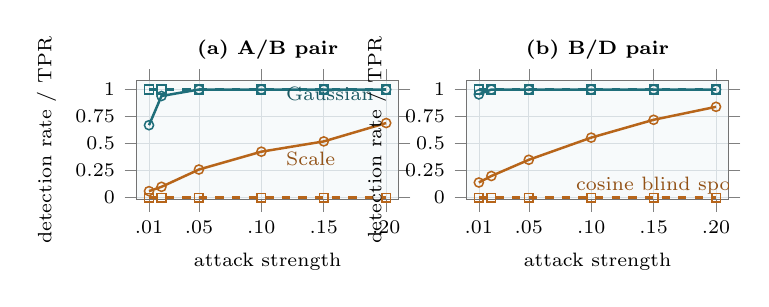
\begin{tikzpicture}
\definecolor{veSweepGaussian}{HTML}{1F6E7A}
\definecolor{veSweepScale}{HTML}{B7651A}
\definecolor{veSweepGrid}{HTML}{D7DEE2}
\definecolor{veSweepPanel}{HTML}{F7FAFB}
\begin{groupplot}[
	group style={group size=2 by 1,horizontal sep=0.86cm},
	width=0.405\textwidth,
	height=0.255\textwidth,
	xmin=0.0,xmax=0.21,
	ymin=-0.02,ymax=1.08,
	xtick={0.01,0.05,0.10,0.15,0.20},
	xticklabels={.01,.05,.10,.15,.20},
	ytick={0,0.25,0.5,0.75,1.0},
	xlabel={attack strength},
	ylabel={detection rate / TPR},
	tick label style={font=\scriptsize},
	label style={font=\scriptsize},
	title style={font=\scriptsize\bfseries,yshift=-0.4ex},
	legend style={
		font=\scriptsize,
		draw=none,
		fill=white,
		fill opacity=0.88,
		text opacity=1,
		row sep=0pt,
		cells={anchor=west}
	},
	grid=major,
	major grid style={draw=veSweepGrid,line width=0.25pt},
	axis background/.style={fill=veSweepPanel},
	axis line style={draw=black!55,line width=0.35pt},
	tick align=outside,
	every axis plot/.append style={line width=0.9pt},
]

\nextgroupplot[
	title={(a) A/B pair},
]
\addplot+[color=veSweepGaussian,solid,mark=o,mark size=1.65pt,
	mark options={solid,fill=white,draw=veSweepGaussian,line width=0.55pt}]
	coordinates {
		(0.01,0.67) (0.02,0.94) (0.05,1.00)
		(0.10,1.00) (0.15,1.00) (0.20,1.00)
	};
\addplot+[color=veSweepGaussian,dashed,mark=square,mark size=1.55pt,
	mark options={solid,fill=white,draw=veSweepGaussian,line width=0.55pt}]
	coordinates {
		(0.01,1.00) (0.02,1.00) (0.05,1.00)
		(0.10,1.00) (0.15,1.00) (0.20,1.00)
	};
\addplot+[color=veSweepScale,solid,mark=o,mark size=1.65pt,
	mark options={solid,fill=white,draw=veSweepScale,line width=0.55pt}]
	coordinates {
		(0.01,0.06) (0.02,0.10) (0.05,0.26)
		(0.10,0.425) (0.15,0.52) (0.20,0.69)
	};
\addplot+[color=veSweepScale,dashed,mark=square,mark size=1.55pt,
	mark options={solid,fill=white,draw=veSweepScale,line width=0.55pt}]
	coordinates {
		(0.01,0.00) (0.02,0.00) (0.05,0.00)
		(0.10,0.00) (0.15,0.00) (0.20,0.00)
	};
\node[anchor=west,font=\scriptsize,text=veSweepGaussian!80!black]
	at (axis cs:0.112,0.96) {Gaussian};
\node[anchor=west,font=\scriptsize,text=veSweepScale!80!black]
	at (axis cs:0.112,0.36) {Scale};

\nextgroupplot[
	title={(b) B/D pair},
]
\addplot+[color=veSweepGaussian,solid,mark=o,mark size=1.65pt,
	mark options={solid,fill=white,draw=veSweepGaussian,line width=0.55pt}]
	coordinates {
		(0.01,0.955) (0.02,1.00) (0.05,1.00)
		(0.10,1.00) (0.15,1.00) (0.20,1.00)
	};
\addplot+[color=veSweepGaussian,dashed,mark=square,mark size=1.55pt,
	mark options={solid,fill=white,draw=veSweepGaussian,line width=0.55pt}]
	coordinates {
		(0.01,1.00) (0.02,1.00) (0.05,1.00)
		(0.10,1.00) (0.15,1.00) (0.20,1.00)
	};
\addplot+[color=veSweepScale,solid,mark=o,mark size=1.65pt,
	mark options={solid,fill=white,draw=veSweepScale,line width=0.55pt}]
	coordinates {
		(0.01,0.14) (0.02,0.20) (0.05,0.35)
		(0.10,0.555) (0.15,0.72) (0.20,0.84)
	};
\addplot+[color=veSweepScale,dashed,mark=square,mark size=1.55pt,
	mark options={solid,fill=white,draw=veSweepScale,line width=0.55pt}]
	coordinates {
		(0.01,0.00) (0.02,0.00) (0.05,0.00)
		(0.10,0.00) (0.15,0.00) (0.20,0.00)
	};
\node[anchor=west,font=\scriptsize,text=veSweepScale!80!black]
	at (axis cs:0.08,0.11) {cosine blind spot};

\end{groupplot}
\end{tikzpicture}
}
\caption{Material-tamper strength sweep. Solid lines are scalar16 and dashed
lines are projcos4; teal denotes Gaussian noise and orange denotes scale
perturbations. The sweep confirms that cosine-only projected-token sketches
detect direction-changing perturbations but remain weak against
direction-preserving scale changes.}
\Description{A TikZ plot showing material-tamper detection rates across attack
strengths for Gaussian and scale perturbations on the A/B and B/D stack pairs.}
\label{fig:app-strength-sweep}
\end{figure*}

\begin{figure*}[t]
\centering
\resizebox{\suppPayloadLatencyWidth}{!}{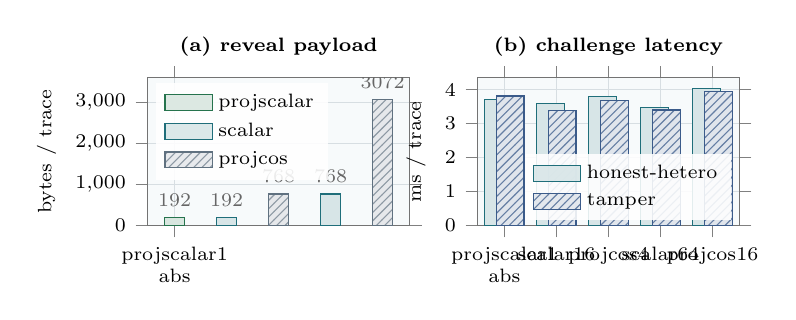
\begin{tikzpicture}
\definecolor{veOverBridge}{HTML}{26734D}
\definecolor{veOverScalar}{HTML}{1F6E7A}
\definecolor{veOverProjcos}{HTML}{607180}
\definecolor{veOverHetero}{HTML}{1F6E7A}
\definecolor{veOverTamper}{HTML}{3B5B8A}
\definecolor{veOverGrid}{HTML}{D7DEE2}
\definecolor{veOverPanel}{HTML}{F7FAFB}
\begin{groupplot}[
	group style={group size=2 by 1,horizontal sep=0.86cm},
	width=0.405\textwidth,
	height=0.285\textwidth,
	symbolic x coords={projscalar,scalar16,projcos4,scalar64,projcos16},
	xtick=data,
	xticklabels={{projscalar1\\abs},scalar16,projcos4,scalar64,projcos16},
	x tick label style={font=\scriptsize,align=center},
	tick label style={font=\scriptsize},
	label style={font=\scriptsize},
	title style={font=\scriptsize\bfseries,yshift=-0.4ex},
	legend style={
		font=\scriptsize,
		draw=none,
		fill=white,
		fill opacity=0.88,
		text opacity=1,
		row sep=0pt,
		cells={anchor=west}
	},
	enlarge x limits=0.13,
	grid=major,
	major grid style={draw=veOverGrid,line width=0.25pt},
	axis background/.style={fill=veOverPanel},
	axis line style={draw=black!55,line width=0.35pt},
	tick align=outside,
]

\nextgroupplot[
	title={(a) reveal payload},
	ylabel={bytes / trace},
	ymin=0,ymax=3600,
	ytick={0,1000,2000,3000},
	legend pos=north west,
]
\addplot+[ybar,bar width=7.2pt,area legend,mark=none,fill=veOverBridge!18,draw=veOverBridge,line width=0.45pt]
	coordinates {(projscalar,192)};
\addlegendentry{projscalar}
\addplot+[ybar,bar width=7.2pt,area legend,mark=none,fill=veOverScalar!18,draw=veOverScalar,line width=0.45pt]
	coordinates {(scalar16,192) (scalar64,768)};
\addlegendentry{scalar}
\addplot+[ybar,bar width=7.2pt,area legend,mark=none,fill=veOverProjcos!16,draw=veOverProjcos,line width=0.45pt,
	postaction={pattern=north east lines,pattern color=veOverProjcos!72}]
	coordinates {(projcos4,768) (projcos16,3072)};
\addlegendentry{projcos}
\node[anchor=south,font=\scriptsize,text=black!60] at (axis cs:projscalar,218) {192};
\node[anchor=south,font=\scriptsize,text=black!60] at (axis cs:scalar16,218) {192};
\node[anchor=south,font=\scriptsize,text=black!60] at (axis cs:projcos4,805) {768};
\node[anchor=south,font=\scriptsize,text=black!60] at (axis cs:scalar64,805) {768};
\node[anchor=south,font=\scriptsize,text=black!60] at (axis cs:projcos16,3110) {3072};

\nextgroupplot[
	title={(b) challenge latency},
	ylabel={ms / trace},
	ymin=0,ymax=4.35,
	ytick={0,1,2,3,4},
	legend pos=south east,
]
\addplot+[ybar=2.8pt,bar shift=-2.1pt,area legend,mark=none,fill=veOverHetero!18,draw=veOverHetero,line width=0.45pt]
	coordinates {
		(projscalar,3.708742) (scalar16,3.603487) (projcos4,3.798230)
		(scalar64,3.468791) (projcos16,4.040801)
	};
\addlegendentry{honest-hetero}
\addplot+[ybar=2.8pt,bar shift=2.1pt,area legend,mark=none,fill=veOverTamper!16,draw=veOverTamper,line width=0.45pt,
	postaction={pattern=north east lines,pattern color=veOverTamper!78}]
	coordinates {
		(projscalar,3.813726) (scalar16,3.381667) (projcos4,3.683724)
		(scalar64,3.402573) (projcos16,3.943448)
	};
\addlegendentry{tamper}

\end{groupplot}
\end{tikzpicture}
}
\caption{Checkpoint-sketch payload and challenge-time verifier latency. Reveal
payload scales with sketch dimensionality, while measured verifier latency
remains in the few-millisecond range across scalar-coordinate, projected-token,
and projected-scalar variants.}
\label{fig:app-payload-latency}
\Description{A TikZ plot comparing checkpoint-sketch reveal payload and
challenge-time verifier latency across TSTC verifier variants.}
\end{figure*}

\begin{figure*}[b]
\centering
\resizebox{\suppPolicyCompareWidth}{!}{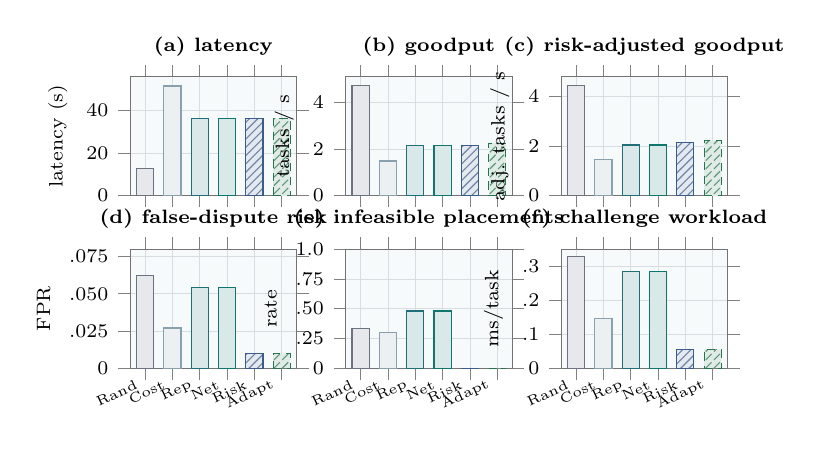
\begin{tikzpicture}
\definecolor{vePolRandom}{HTML}{6B7280}
\definecolor{vePolCost}{HTML}{8AA0AD}
\definecolor{vePolRep}{HTML}{1F6E7A}
\definecolor{vePolNet}{HTML}{0F766E}
\definecolor{vePolRisk}{HTML}{3B5B8A}
\definecolor{vePolAdapt}{HTML}{26734D}
\definecolor{vePolGrid}{HTML}{D7DEE2}
\definecolor{vePolPanel}{HTML}{F7FAFB}
\newcommand{\vePolicySolidBar}[2]{%
	\addplot+[ybar,bar width=6.2pt,mark=none,fill=#1!16,draw=#1,line width=0.4pt]
		coordinates {#2};%
}
\newcommand{\vePolicyHatchBar}[2]{%
	\addplot+[ybar,bar width=6.2pt,mark=none,fill=#1!14,draw=#1,line width=0.4pt,
		postaction={pattern=north east lines,pattern color=#1!74}] coordinates {#2};%
}
\begin{groupplot}[
	group style={group size=3 by 2,horizontal sep=0.62cm,vertical sep=0.68cm},
	width=0.305\textwidth,
	height=0.255\textwidth,
	symbolic x coords={Rand,Cost,Rep,Net,Risk,Adapt},
	xtick={Rand,Cost,Rep,Net,Risk,Adapt},
	xticklabels={Rand,Cost,Rep,Net,Risk,Adapt},
	x tick label style={font=\tiny,rotate=25,anchor=east},
	tick label style={font=\scriptsize},
	label style={font=\scriptsize},
	title style={font=\scriptsize\bfseries,yshift=-0.5ex},
	enlarge x limits=0.11,
	grid=major,
	major grid style={draw=vePolGrid,line width=0.25pt},
	axis background/.style={fill=vePolPanel},
	axis line style={draw=black!55,line width=0.35pt},
	tick align=outside,
]

\nextgroupplot[
	title={(a) latency},
	ylabel={latency (s)},
	ymin=0,ymax=56,
	ytick={0,20,40},
	xticklabels={,,,,,},
]
\vePolicySolidBar{vePolRandom}{(Rand,12.781498)}
\vePolicySolidBar{vePolCost}{(Cost,51.636917)}
\vePolicySolidBar{vePolRep}{(Rep,36.310436)}
\vePolicySolidBar{vePolNet}{(Net,36.310436)}
\vePolicyHatchBar{vePolRisk}{(Risk,36.310436)}
\vePolicyHatchBar{vePolAdapt}{(Adapt,36.310436)}

\nextgroupplot[
	title={(b) goodput},
	ylabel={tasks / s},
	ymin=0,ymax=5.1,
	ytick={0,2,4},
	xticklabels={,,,,,},
]
\vePolicySolidBar{vePolRandom}{(Rand,4.741068)}
\vePolicySolidBar{vePolCost}{(Cost,1.485707)}
\vePolicySolidBar{vePolRep}{(Rep,2.160597)}
\vePolicySolidBar{vePolNet}{(Net,2.160597)}
\vePolicyHatchBar{vePolRisk}{(Risk,2.160597)}
\vePolicyHatchBar{vePolAdapt}{(Adapt,2.240619)}

\nextgroupplot[
	title={(c) risk-adjusted goodput},
	ylabel={adj. tasks / s},
	ymin=0,ymax=4.8,
	ytick={0,2,4},
	xticklabels={,,,,,},
]
\vePolicySolidBar{vePolRandom}{(Rand,4.445107)}
\vePolicySolidBar{vePolCost}{(Cost,1.445593)}
\vePolicySolidBar{vePolRep}{(Rep,2.043924)}
\vePolicySolidBar{vePolNet}{(Net,2.043924)}
\vePolicyHatchBar{vePolRisk}{(Risk,2.139855)}
\vePolicyHatchBar{vePolAdapt}{(Adapt,2.219109)}

\nextgroupplot[
	title={(d) false-dispute risk},
	ylabel={FPR},
	ymin=0,ymax=0.08,
	ytick={0,0.025,0.05,0.075},
	scaled y ticks=false,
	yticklabels={0,.025,.050,.075},
]
\vePolicySolidBar{vePolRandom}{(Rand,0.062425)}
\vePolicySolidBar{vePolCost}{(Cost,0.027000)}
\vePolicySolidBar{vePolRep}{(Rep,0.054000)}
\vePolicySolidBar{vePolNet}{(Net,0.054000)}
\vePolicyHatchBar{vePolRisk}{(Risk,0.009600)}
\vePolicyHatchBar{vePolAdapt}{(Adapt,0.009600)}

\nextgroupplot[
	title={(e) infeasible placements},
	ylabel={rate},
	ymin=0,ymax=1.0,
	ytick={0,0.25,0.50,0.75,1.0},
	yticklabels={0,.25,.50,.75,1.0},
]
\vePolicySolidBar{vePolRandom}{(Rand,0.335)}
\vePolicySolidBar{vePolCost}{(Cost,0.300)}
\vePolicySolidBar{vePolRep}{(Rep,0.480)}
\vePolicySolidBar{vePolNet}{(Net,0.480)}
\vePolicyHatchBar{vePolRisk}{(Risk,0.000)}
\vePolicyHatchBar{vePolAdapt}{(Adapt,0.000)}

\nextgroupplot[
	title={(f) challenge workload},
	ylabel={ms/task},
	ymin=0,ymax=0.35,
	ytick={0,0.1,0.2,0.3},
	yticklabels={0,.1,.2,.3},
]
\vePolicySolidBar{vePolRandom}{(Rand,0.327945)}
\vePolicySolidBar{vePolCost}{(Cost,0.145264)}
\vePolicySolidBar{vePolRep}{(Rep,0.284592)}
\vePolicySolidBar{vePolNet}{(Net,0.284592)}
\vePolicyHatchBar{vePolRisk}{(Risk,0.054005)}
\vePolicyHatchBar{vePolAdapt}{(Adapt,0.054005)}

\end{groupplot}
\end{tikzpicture}
}
\caption{Queued-workload policy comparison. The plot shows the tradeoff among
modeled latency, goodput, risk-adjusted goodput, false-dispute risk,
infeasible usage, and expected challenge workload; Risk and Adapt. denote the
risk-constrained and adaptive-verifier policies.}
\label{fig:app-placement-policy-compare}
\Description{A TikZ plot comparing queued-workload placement policies by
latency, goodput, risk-adjusted goodput, false-dispute risk, infeasible
placement rate, and expected challenge workload.}
\end{figure*}

\clearpage
\end{document}
